\chapter{Sample Manager Page}
Samples can be transferred to and received from the Machinedrum via the Sample Manager Page. Two file types are supported: 
\begin{enumerate}
    \item \textbf{WAV} -- (UW models only) $.wav$ PCM samples.
    \item \textbf{SYSEX} -- (UW models only) $.syx$ Midi SDS samples, this is the format of the official Machinedrum sound packs.
\end{enumerate}

\screenshot{sample_manager.png}
\textit{To enter the Sound Manager Page: press and hold \textbf{[Global]}, then press \textbf{[Trig 9]}.}

\section{Navigating the Sound Browser Page}


%\fbox{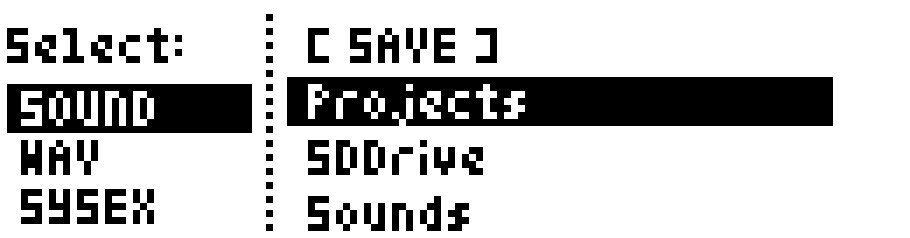
\includegraphics[scale=.40]{sound_page.png}}
\screenshot{sample_browser_page.png}
\begin{itemize}
    \item Use the \textbf{[Up]} and \textbf{[Down]} arrow keys to scroll through.
    \item Press \textbf{<Enter/Yes>} to enter a directory, or load a sound to the current track.
    \item Press \textbf{<Exit/No>} to exit/cancel.
    \item Press and hold \textbf{<Global>} to create a new folder, delete or rename a sound.
\end{itemize}

Note that the Sample Manager will filter the directory content for $.wav$ $.syx$ file types.
\newpage
\section{Receiving Samples}
To receive a \textbf{WAV} sample from the MD:
\begin{enumerate}
    \item Select [RECV].
    \item The file browser panel will now display the sample slots in the MD, with ROM slots first, and RAM slots (shown as R1-R4) in the end.
    \item Select the slot to receive sample from.
    \item The SDS dump will be converted to a PCM wave file on the fly, and saved to the current folder on the micro SD card.
\end{enumerate}

\section{Transferring Samples}
To transfer, select the file the from the Sample Manager. The display will now show the ROM slots availble in the MD, and you can select one slot to send the sample to.
\screenshot{rom_select.png}
\section{Bulk Sample Load and Receive}
To send or receive multiple WAVs, press and hold \textbf{[Global]} to access the \textbf{Send All / Recv All} functions which will transfer files from/to the current folder.
\begin{itemize}
\item When receiving, samples are saved to the current directory.
\item Sample names are prefixed with a 2 digit slot number. This 2 digit number is used to preserve sample order when re-uploading. (Therefore, ROM positions can be saved and recalled for each project.)
\item Sample names that do not start with a slot number will be excluded from bulk upload.
\end{itemize}
\section{Cancelling Transfer}
Sample transfers between can be cancelled by pressing the MD's \textbf{[No]} key.
\newpage
\section{Delete or Rename Samples}
\screenshot{file_menu.png}
\textit{From within the Sample Manager, press and hold \textbf{[Global]} to access the file options menu.}\\\\
From the file options menu, you may delete or rename sound files or create new directories.\\\\
Use the encoder to make your selection, release \textbf{[Global]} to activate your choice.
\section{Preparing and Transferring Files With a Computer}
Using an appropriate adaptor, you can mount the SD card as a drive on your computer. \\
\\
\textbf{WAV} files must meet the following requirements:
\begin{itemize}
    \item Filename up to 31 characters including extension. (When loaded into ROM, MD will truncate this to the first two and last two characters of the filename before the extension.)
    \item Sample speeds from 4kHz to 48kHz, ideally 44100Hz or 22050Hz to avoid resampling
    \item Any bit depth is accepted (MD stores samples at 12bit)\newline
\end{itemize}
\
MD UW only plays back mono samples.